\documentclass[11pt]{article}
\usepackage[utf8]{inputenc}
%\usepackage[T1]{fontenc}
\usepackage{amssymb}
\usepackage{amsmath}
\usepackage{enumerate}
\usepackage{fullpage}
\usepackage{polski}  
\usepackage{indentfirst} 
\usepackage[pdftex]{graphicx}
\usepackage{multirow}
\usepackage{placeins}
\usepackage{wasysym}
\usepackage{xspace}
\usepackage{import}
\usepackage{multicol}

\begin{document}
\begin{center}
\begin{tabular}{|c|c|c|c|c|}
\hline
Wydział & \underline{Łukasz Dubiel} & Rok & Grupa & Cw. nr \\
%\hline
EAIE & Daniel Iziorov, Piotr Mędrek & I & Grupa 6 & 1 \\
\hline
Data wykoania & \multicolumn{3}{|l|}{Temat} & Ocena \\
2.03.2012 &  \multicolumn{3}{|p{10.5cm}|}{Charakterystyki stffałoprądowe złącza p-n. diody prostownicze i specjalne} & \\
\hline
\end{tabular}
\end{center}

\section{Pomiary charakterysytk diod w kierunku przewodzenia}

\subsection{Diody prostownicze}
Zebrane charakterystyki
\begin{center}
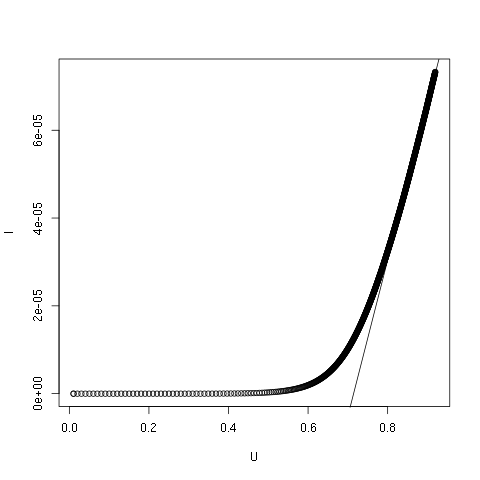
\includegraphics[scale=0.45]{out/prostownicza-normal.png}
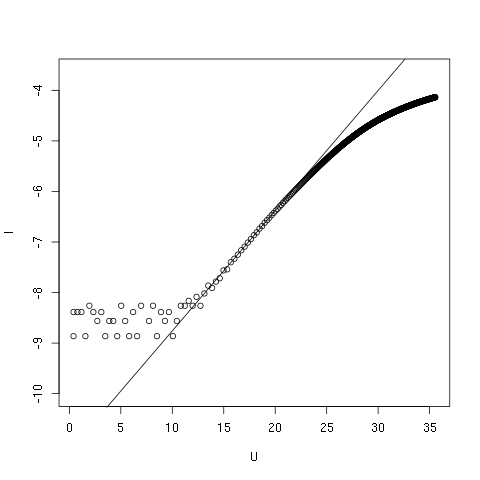
\includegraphics[scale=0.45]{out/prostownicza-log.png}
\end{center}
Ogólne równanie diody
$$ i_d = I_{gr0}(e^{\frac{u_d - r_di_d}{U_t}} - 1) + I_0(e^{\frac{u_d - r_di_d}{U_t}} -1) $$
Dla $ U_f > 100mV$ można przująć przybliżenie
$$ i_D = I_se^\frac{u_d}{nU_t} $$

Napięcie progowe wynosi
$$ U_k =  0.7144 $$

Fragmenty małych prądów i rekombinacyjny jest bardzo mały w charakterystyce, wynika z tego mocno dyfuzyjny charakter diody.
W uzyskanej charakterystyce można wyznaczyć trzy obszary. Gdy $\frac{U}{U_t} \in <16,20>$ dioda pracuje w obszarze dominacji prądu dyfuzyjnego. Gdy $\frac{U}{U_t} \in <20,27>$ obszar pracy przechodzi do obszaru prądów unoszenia. Powyżej znajduje się obszar omowy.

Używając metody regresji lniowej na obszarze dyfuzyjnym uzykujemy wynik
$$ a =  0.2378 \quad b = -11.137 $$

Charakterystyka pół logartymiczn w obszarze dyfuzujnym odpowiada
$$ \ln{I_d} = \frac{u_d}{nU_t} + I_0$$
Co daje równość
$$ a = \frac{1}{n} \quad b = I_0 $$

Czyli odpowiednie wartośći są równe
$$ n = 4,20 \quad I_0 = 14,5 \mu A $$

Gdzie $n$ to współczynnik niedoskonałości łącza, a $I_0$ to wartość prądu dyfuzyjnego

Wiadomym jest że $ I_0 < I_{GR0} $ tak więc, dla przyjętnego uproszczonego równia współczynik 
$$ I_s = I_0 $$
$$ I_s = 14,5 \mu A $$

Rezystancja szeregowa wynosi
$$ r_s = \frac{\Delta U}{I_d} = \frac{U_d - U_k}{I_d} $$
Obliczenia wykonane dla prądu $20mA$
$$ r_s = \frac{0,756-0.7144}{0.02} = 2.08 \Omega $$

\section{Dioda germanowa}
Charakterystyki 
\begin{center}
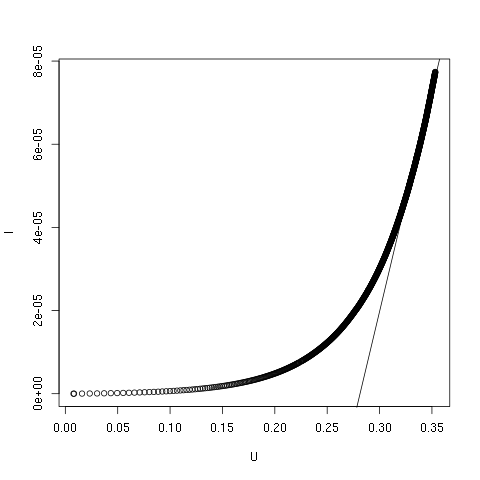
\includegraphics[scale=0.48]{out/germanowa-normal.png}
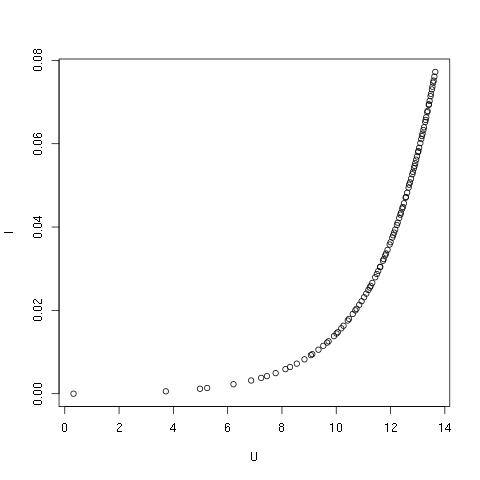
\includegraphics[scale=0.48]{out/germanowa-log.png}
\end{center}
\begin{description}
\item[Napięcie progowe $U_k$] $=0,218\ V$
\item[Współczynnik niedoskońałośći złącza $n$]  $=3.899$
\item[Prąd dyfuzyjny $I_0$ ] $=796\ \mu A$
\item[Rezystancja szeregowa ($I=75mA$) $r_s$ ] $=0,934\ \Omega$
\end{description}
\section{Dioda impulsowa}
Charakterystyki 
\begin{center}
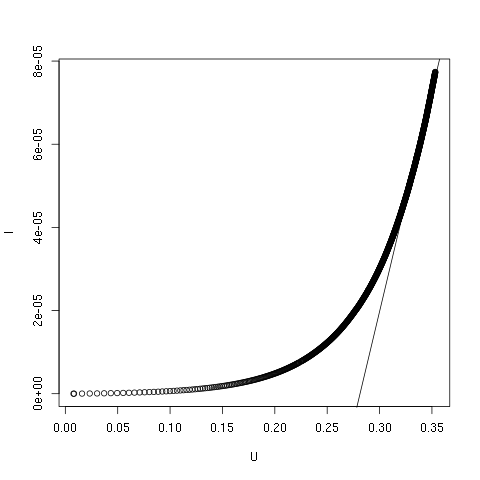
\includegraphics[scale=0.48]{out/germanowa-normal.png}
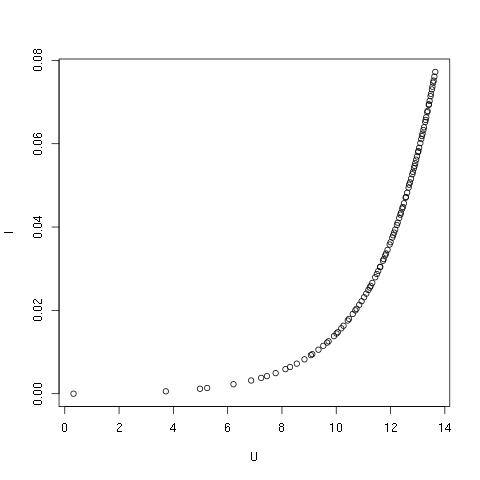
\includegraphics[scale=0.48]{out/germanowa-log.png}
\end{center}
\begin{description}
\item[Napięcie progowe $U_k$] $=0,7477\ V$
\item[Współczynnik niedoskońałośći złącza $n$]  $=4,2542$
\item[Prąd dyfuzyjny $I_0$ ] $=73\ \mu A$
\item[Rezystancja szeregowa ($I=73mA$) $r_s$ ] $=1,924\ \Omega$
\end{description}
\newpage
\includegraphics[scale=0.9]{out/diody-all.png}
Z pary bliko siedzie bardziej nachylony należy do diody impulsowej.
\subsection{Wnioski}
Charakterystyka bardzo mocno zależy od materiału diody. Widać znaczną róznicę między diodą germanową a krzemowymi. Rówież samo wykonanie diody oraz preferowane zastosowanie (w przypadku diody impulsowej układy w.cz.) wpływają na jej charakterystyki napięciowo-prądowe.
\section{Diody stabilizacyjne}
\begin{center}
\includegraphics[scale=0.48]{out/stabilizacja.png}
\end{center}
\subsection{Rezystancja dynamiczna}
\begin{center}
\begin{tabular}{|c|c|c|c|}
\hline
Dioda & $0,1mA$ & $1mA$ & $10mA$ \\
\hline
$3,6V$ & $1000 \Omega$ & $350 \Omega$ & $60 \Omega$ \\
\hline
$5,4V$ & $1250 \Omega$ & $386 \Omega$ & $26,98 \Omega$ \\
\hline
$7,5V$ & $4936.5 \Omega$ & $53 \Omega$ & $39,27 \Omega$ \\
\hline
\end{tabular}
\end{center}
Różnice w charakterystyce kształcie charektyrystk jak również w wartościach
rezystancji dynamicznej wynikają z całkwitej domiennośći zajawisk fizycznych
działających w diodzie.

Dla diod o niskim napięciu ($3,6V$;$5,4V$) dominującym zjawiskiem jest efekt Zennera. Dla diod o wysokim napięciu stabilizacji zajwiskiem odpowiedialnyum za przeowdzenie diody jest przebicie lawinowe.
To właśnie ono powoduje posiadanie tak znacznej rezystancji dynamicznej dla małych prądów oraz szybki jej spadem wraz wzrostem płynącego prądu.

Diody o przebiciu opierające swoje działanie o effekt zenner posiadają lepsze właściwości stabilizacyjne ze względu na bardziej stomą charakterystykę. Dzięki temu trzymają się bliżej zadanego napięcia. Argumentem za tym są niskie wartości rezystancji dynamicznej 

\section{Diody LED}
\begin{center}
\includegraphics[scale=0.48]{out/led-normal.png}
\end{center}
Napięcia na diodach przy prądzie $1mA$
\begin{center}
\begin{tabular}{|c|c|c|c|c|}
  \hline
  $I_d$ & Biała & Żółta & Zielona & Pomarańczowa \\
  \hline
  $1mA$ & $2,9V$ & $1,76V$& $1,8V$ & $1,77V$ \\
  \hline
\end{tabular}
\end{center}

\subsection{Wnioski}
Diody posiadają rożne napięcie dzialania w zależności od koloru światła. Powodowane jest to różnymi materiałami służacymi do ich budowy i uzyskania światła. Jendak w przypadku większości kolorów punkt zadziałania jest bardzo blisko siebie ($1,77V$) 
\end{document}
